% !TEX root = ../Thesis.tex
\begin{document}
\documentclass[Thesis.tex]{subfiles}
\chapter{Fine-grained information presentation}
\label{ch:infpres}



%To be able to show or hide specific parts of the letters we try to break them apart into useful sections. (Irgendwie kein runder Übergang. Bin mir auch nicht ganz sicher, ob der nächste Teil noch in die Intro gehört. Macht aber schon Sinn, dann kann ich im nächsten Kapitel gleich mit einer Anwendung anfangen, für die ich alle anderen Methoden einführen muss.)



\section{Paragraph Extraction}

As already mentioned above, the letters almost always contain separate
paragraphs like greeting, diagnosis, therapy history and anamnesis.
To be able to hide unnecessary information or to only present requested
information it is useful to automatically extract individual
paragraphs from the documents. As the documents are similar in structure
and the word XML format allows to automatically examine the XML tree
structure of a document, we use a rule based approach for extracting
the individual paragraphs. A simplified rule to find the beginning of the diagnosis paragraph is shown in pseudocode:
%\bigskip
%
%\begin{algorithm}[H]
%	\DontPrintSemicolon
%	diagnosisRegex = '[dD]iagnose(n)?'\;
%	text = thisXmlNode.text()\;
%	\If{regex.match(text, diagnosisRegex)
%		$ {\bf and} $ boldface(text)
%		$ {\bf and} $ precededByNewline(thisXmlNode)}{
%		diagnosisStart = thisXmlNode\;
%		}
%		
%		\caption{Simplified pseudocode algorithm to find the beginning of the diagnosis paragraph}
%\end{algorithm}
%		
%\bigskip
\bigskip

\begin{lstlisting}
diagnosis_regex = '[dD]iagnose(n)?'
text = this_xml_node.text()
if diagnosis_regex.match(text)
	and boldface(text)
	and preceded_by_newline(this_xml_node):
then:
	diagnosis_start = this_xml_node
\end{lstlisting}

\bigskip
%(Weder der erste noch der zweite pseudocode gefällt mir bis jetzt. Wird noch geändert.)

A regular expression is defined that matches the beginning of the diagnosis paragraph (the German word for diagnosis is "Diagnose").
The text of every node in the XML tree is checked for a regular expression match and several other rules. If an XML node matches all criteria it is marked as the beginning of the diagnosis paragraph.
With a set of rules like the one above we automatically extract the
paragraphs of interest from the documents. This approach, however,
is not completely reliable, as the doctors are free to write the documents
in the way they please. Indeed we find several wrongly extracted paragraphs,
that e.g. include the subsequent paragraph as well. For our dataset
it is possible to check the extraction process by hand. However, this
is tedious work and is not scalable to bigger
datasets. We therefore explore whether we can in principle make use
of other automated methods to find paragraphs for which the extraction
process does not produce desired results. We therefore take several correctly extracted and one incorrectly extracted
diagnosis paragraphs and convert them to their bag of words representation.
To get a feeling for how these vectors behave we use Principle Component
Analysis (PCA) to get a lower dimensional approximation of the vectors. PCA finds the linear
subspace with desired dimensionality of the original space that preserves as much of the variance of the vectors in the original space as possible. Thereby one can gain a low dimensional approximation of the high dimensional data and use this approximation for visual inspection.
See figure \ref{fig:bow_find_odd} for a 2D PCA plot of the bag of words representation
of the correctly and incorrectly extracted diagnose paragraph. As is apparent from the figure, it would not be a
hard task to automatically detect the outlier. In this case the incorrectly
extracted paragraph includes not only the diagnosis, but also the
therapy history. In cases like this with additional text present, it is an easy task to
identify the incorrect ones. A harder problem arises, when only parts
of the paragraph of interest have been extracted. However, we believe
that this problem is of little concern. The way our rules are built it
is very unlikely that we will face this problem. The paragraph would
have to include an empty line, the subsequent one would have to contain
only boldface characters and a few more conditions would have to be
fulfilled for this problem to arise. Indeed, we did not find a case
of this problem in our dataset. (Ich könnte auch mal tatsächliche outlier detection machen, wenn du das für sinnvoll hälst. Hab ein paar Ideen, die gut funktionieren könnten, wollte aber keine Zeit rein stecken, falls wir es nicht benutzen wollen.)
\begin{figure}
	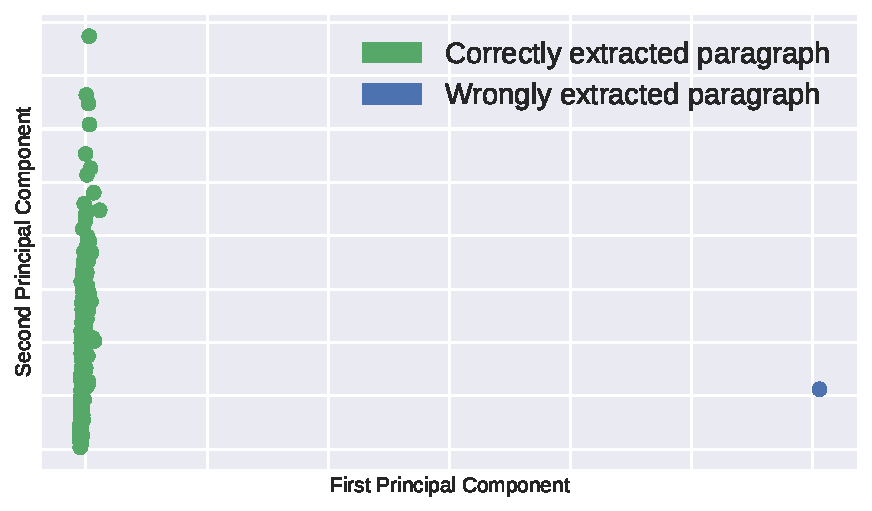
\includegraphics[width=\linewidth]{figures/bow_find_odd}
	\caption{2D PCA projection of bag of words representation of one incorrectly extracted diagnosis paragraph and several correctly extracted ones.}
	\label{fig:bow_find_odd}
\end{figure}

\end{document}